\documentclass[11pt]{article}
\usepackage{import}
\usepackage[margin=1in, top=1in]{geometry}
\usepackage[all]{nowidow}
\usepackage[hyperfigures=true, hidelinks, pdfhighlight=/N]{hyperref}
\usepackage[separate-uncertainty=true, group-digits=false]{siunitx}
\usepackage{graphicx,amsmath,physics,tabto,float,amssymb,pgfplots,verbatim,tcolorbox}
\usepackage{listings,xcolor,subfig,caption,import,wrapfig,lipsum,tikz,biblatex}
\usepackage[version=4]{mhchem}
\usepackage[noabbrev]{cleveref}
\newcommand{\creflastconjunction}{, and\nobreakspace}
\newcommand{\mb}[1]{\mathbf{#1}}
\numberwithin{equation}{section}
\numberwithin{figure}{section}
\numberwithin{table}{section}
\definecolor{stringcolor}{HTML}{C792EA}
\definecolor{codeblue}{HTML}{2162DB}
\definecolor{commentcolor}{HTML}{4A6E46}
\captionsetup{font=small, belowskip=0pt}
\lstdefinestyle{appendix}{
    basicstyle=\ttfamily\footnotesize,commentstyle=\color{commentcolor},keywordstyle=\color{codeblue},
    stringstyle=\color{stringcolor},showstringspaces=false,numbers=left,upquote=true,captionpos=t,
    abovecaptionskip=12pt,belowcaptionskip=12pt,language=Python,breaklines=true,frame=single}
\lstdefinestyle{inline}{
    basicstyle=\ttfamily\footnotesize,commentstyle=\color{commentcolor},keywordstyle=\color{codeblue},
    stringstyle=\color{stringcolor},showstringspaces=false,numbers=left,upquote=true,frame=tb,
    captionpos=b,language=Python}
\renewcommand{\lstlistingname}{Appendix}
\pgfplotsset{compat=1.17}
\addbibresource{bibliography.bib}

\title{{\Huge A ``look-see'' at data from Run 3 at ALICE}}
\author{{\Large Miles Kidson}\\ \\
Supervisors: Prof. Zinhle Buthelezi, Dr. SV Fortsch, \& Prof. Tom Dietel\\
Assisted By: Dr. B Naik (Postdoctoral fellow)}
\date{\textbf{UCT Honours 2022}}

\begin{document}
    
\maketitle

\begin{figure}[h]
    \begin{center}
        
\includegraphics{Figs/UCT.jpg}
    \end{center}
\end{figure}

\begin{abstract}
    \centering
    We investigate pilot-beam data from proton-proton collisions in Run 3 at ALICE, checking if the new Muon Forward Tracker, Inner Tracking System, and Online-Offline analysis framework are working as intended. 
\end{abstract}

\newpage
\tableofcontents

\newpage
\section{Introduction}\label{sec:Introduction}
Run 3 is the latest period of data capture at the LHC, with an intended centre of mass energy per collision of $\sqrt{s}=\SI{13.6}{\tera\electronvolt}$ and increased luminosity of collisions---a factor 10 increase in integrated luminosity for Pb-Pb collisions. For Run 3, ALICE is moving from a triggered readout system to a combination of triggered and continuous readout. In order to achieve this, many detectors and their front-end electronics were upgraded, some new detectors were added, and the analysis framework was overhauled entirely. 

The Inner Tracking System (ITS) was upgraded with an entirely new pixel detector technology, hoping to greatly increase the resolution when determining the primary collision vertex. The Muon Forward Tracker (MFT) is one of the new detectors added. Its primary use is to assist the Muon Spectrometer (MCH) with vertexing and tracking in the forward region of ALICE and was developed with the same technology as the ITS. To deal with the increased volumes of data, a new analysis framework was introduced called Online-Offline (O2).

This report aims to use O2 to have a ``look-see'' at data coming from the ITS and MFT to see if the detector and analysis tools are working correctly. The data used in this investigation is from two proton-proton collision runs performed in October 2021, at a centre-of-mass energy of \SI{900}{\giga\electronvolt}. This is not an energy we expect to use for physics data analysis but is good enough for this purpose.

\section{Background}\label{sec:Background}
\subsection{The ALICE Detector}
\begin{itemize}
    \item What is the LHC?
    \item What is ALICE?
    \item What does ALICE look for?
    \item What is Run 3?
\end{itemize}
The ALICE detector (A Large Ion Collider Experiment) is a detector experiment at the Large Hadron Collider (LHC) at CERN. Its primary goal is the investigation of ``strongly interacting matter at extreme energy densities, where a formation of a new phase of matter, the quark-gluon plasma, is expected'' (\cite{ALICE_LOI}). It achieves this goal by studying the products of head-on collisions of heavy ions such as lead. 

% ALICE is situated at 

% The LHC at CERN in Geneva is built to accelerate particles up to very high energies (\SI{13.6}{\tera\electronvolt})

The coordinate system used at ALICE needs to be discussed first in order to fully explain the scope of this report. A modified cylindrical coordinate system is used as most detectors in the experiment are cylindrically symmetric about the beamline of the LHC. We place the $z$-axis along the beamline and call the angle around the $z$-axis $\varphi$, the azimuthal angle. The angle from the $z$-axis to the $x-y$ plane is called $\theta$, the polar angle. 
We are interested in the momentum of particles that we track in the detector, which we call $\vec{p}$, but we also define the transverse momentum $p_{\mathrm{T}}=\sqrt{p_x^2 + p_y^2}$. The last important coordinate to discuss is the rapidity, often denoted as $y$. This is defined as 
\begin{equation}
    y=\frac 12 \ln\left(\frac{E+p_z}{E-p_z}\right)
    \label{eqn:rapidity}
\end{equation}
where $E$ is the total energy of the particle being considered

\begin{figure}[h]
    \begin{center}
        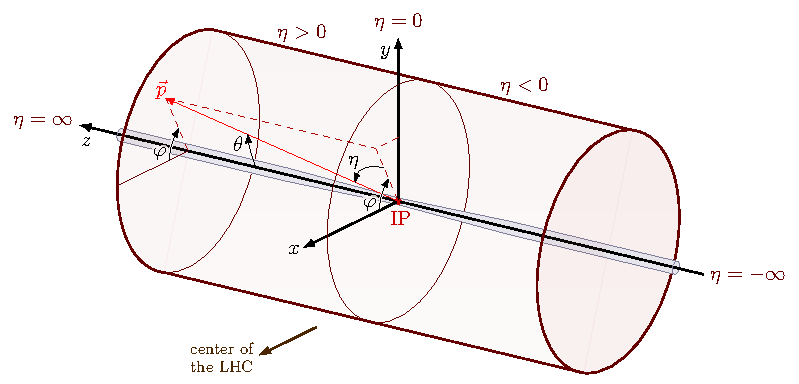
\includegraphics[width=.8\textwidth]{Figs/coords.pdf}
        \caption{Coordinate system \cite{coords}}
        \label{fig:coords}
    \end{center}
\end{figure}


\subsection{Run 3 Specifics}
\begin{itemize}
    \item What was upgraded/added in Run 3?
    \item 
\end{itemize}

\subsection{Muon Forward Tracker}


\section{First Attempts}\label{sec:FirstAttempts}


\newpage
\printbibliography

\end{document}


